\hypertarget{strain_8cpp}{\section{strain.\-cpp \-File \-Reference}
\label{d7/db1/strain_8cpp}\index{strain.\-cpp@{strain.\-cpp}}
}


\-Definition of the member functions if the \hyperlink{classStrain}{\-Strain} class.  


{\ttfamily \#include \char`\"{}strain.\-h\char`\"{}}\*
\-Include dependency graph for strain.\-cpp\-:\nopagebreak
\begin{figure}[H]
\begin{center}
\leavevmode
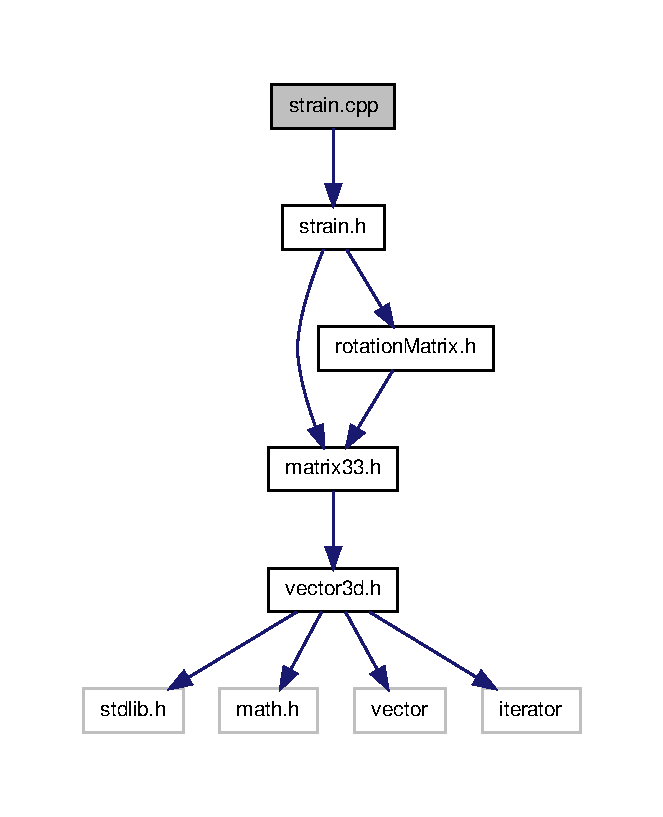
\includegraphics[width=318pt]{d1/da4/strain_8cpp__incl}
\end{center}
\end{figure}


\subsection{\-Detailed \-Description}
\-Definition of the member functions if the \hyperlink{classStrain}{\-Strain} class. \begin{DoxyAuthor}{\-Author}
\-Adhish \-Majumdar 
\end{DoxyAuthor}
\begin{DoxyVersion}{\-Version}
1.\-0 
\end{DoxyVersion}
\begin{DoxyDate}{\-Date}
05/06/2013
\end{DoxyDate}
\-This file defines the member functions of the \hyperlink{classStrain}{\-Strain} class for the strain tensor. 

\-Definition in file \hyperlink{strain_8cpp_source}{strain.\-cpp}.

